\documentclass[12pt,a4paper]{article}
\usepackage[legalpaper, portrait, margin=2cm]{geometry}
\usepackage[portuguese]{babel}
\usepackage[utf8]{inputenc}
\usepackage{fancyhdr}
\usepackage{graphicx}
\usepackage{hyperref}
\usepackage{indentfirst}
\usepackage{listings}
\usepackage{xcolor}

\graphicspath{ {./} }
\hypersetup{
  colorlinks=true,
  linkcolor=blue,
  filecolor=magenta,
  urlcolor=blue,
  citecolor=blue,
  pdftitle={Exercício 1 - Projeto Computacional PE 2022/2023 LEIC-A},
  pdfpagemode=FullScreen,
}

\pagenumbering{gobble}
\pagestyle{fancy}
\fancyhf{}
\rhead{Grupo \textbf{11}}
\lhead{Exercício 1 - Projeto Computacional PE 2022/2023 LEIC-A}
\cfoot{Gonçalo Bárias (103124), Raquel Braunschweig (102624) e Vasco Paisana (102533)}

\renewcommand{\footrulewidth}{0.2pt}

\renewcommand{\labelitemii}{$\circ$}
\renewcommand{\labelitemiii}{$\diamond$}

\definecolor{codegreen}{rgb}{0,0.6,0}
\definecolor{codegray}{rgb}{0.3,0.3,0.3}
\definecolor{codepurple}{rgb}{0.58,0,0.82}

\lstdefinestyle{mystyle}{
  commentstyle=\color{codegreen},
  numberstyle=\tiny\color{codegray},
  % keywordstyle=\color{magenta},
  % stringstyle=\color{codepurple},
  basicstyle=\ttfamily\footnotesize,
  breakatwhitespace=false,
  breaklines=true,
  captionpos=b,
  keepspaces=true,
  numbers=left,
  numbersep=5pt,
  showspaces=false,
  showstringspaces=false,
  showtabs=false,
  tabsize=2
}
\lstset{style=mystyle}

\begin{document}

% Introdução sobre o exercício em questão
O objetivo deste exercício é o de representar, através de um gráfico, a taxa de poupança pessoal e o número de desempregados (em milhares)
para os anos superiores ou iguais a 1996, a partir de um conjunto de dados fornecido pela empresa \href{https://fred.stlouisfed.org/}{FRED}.
Para tal, recorreu-se ao seguinte trecho de código em \texttt{R} (utilizando as bibliotecas \texttt{openxlsx}, \texttt{ggplot2} e \texttt{dplyr}):

\quad

% Código em R para resolver o exercício
\begin{lstlisting}[language=R]
library("openxlsx")
library("ggplot2")
library("dplyr")

df <- read.xlsx(
  xlsxFile = "econ.xlsx", sheet = 1,
  cols = c(1, 4, 6), detectDates = TRUE
)
df_filtered <- df %>% filter(tempo >= "1996-01-01")

normalize_vector <- function(vector) {
    len <- length(vector)
    mean <- mean(vector)
    standard_deviation <- sd(vector)
    for (i in 1:len) {
        vector[i] = (vector[i] - mean) / standard_deviation
    }
    return(vector)
}
df_filtered$tpp <- normalize_vector(df_filtered$tpp)
df_filtered$ndesemp <- normalize_vector(df_filtered$ndesemp)

ggplot(df_filtered, aes(tempo)) +
  geom_line(aes(y = ndesemp, colour = "ndesemp")) +
  geom_line(aes(y = tpp, colour = "tpp")) +
  xlab("Ano") +
  ylab("Variáveis normalizadas") +
  ggtitle("Evolução do Número de Desempregados (ndesemp) e Taxa de Poupança Pessoal (tpp)") +
  labs(colour = "Variáveis", subtitle = "Dados para anos superiores ou iguais a 1996")
\end{lstlisting}

\quad

% Gráfico para resolver o exercício
\begin{figure}[h]
  \centering
  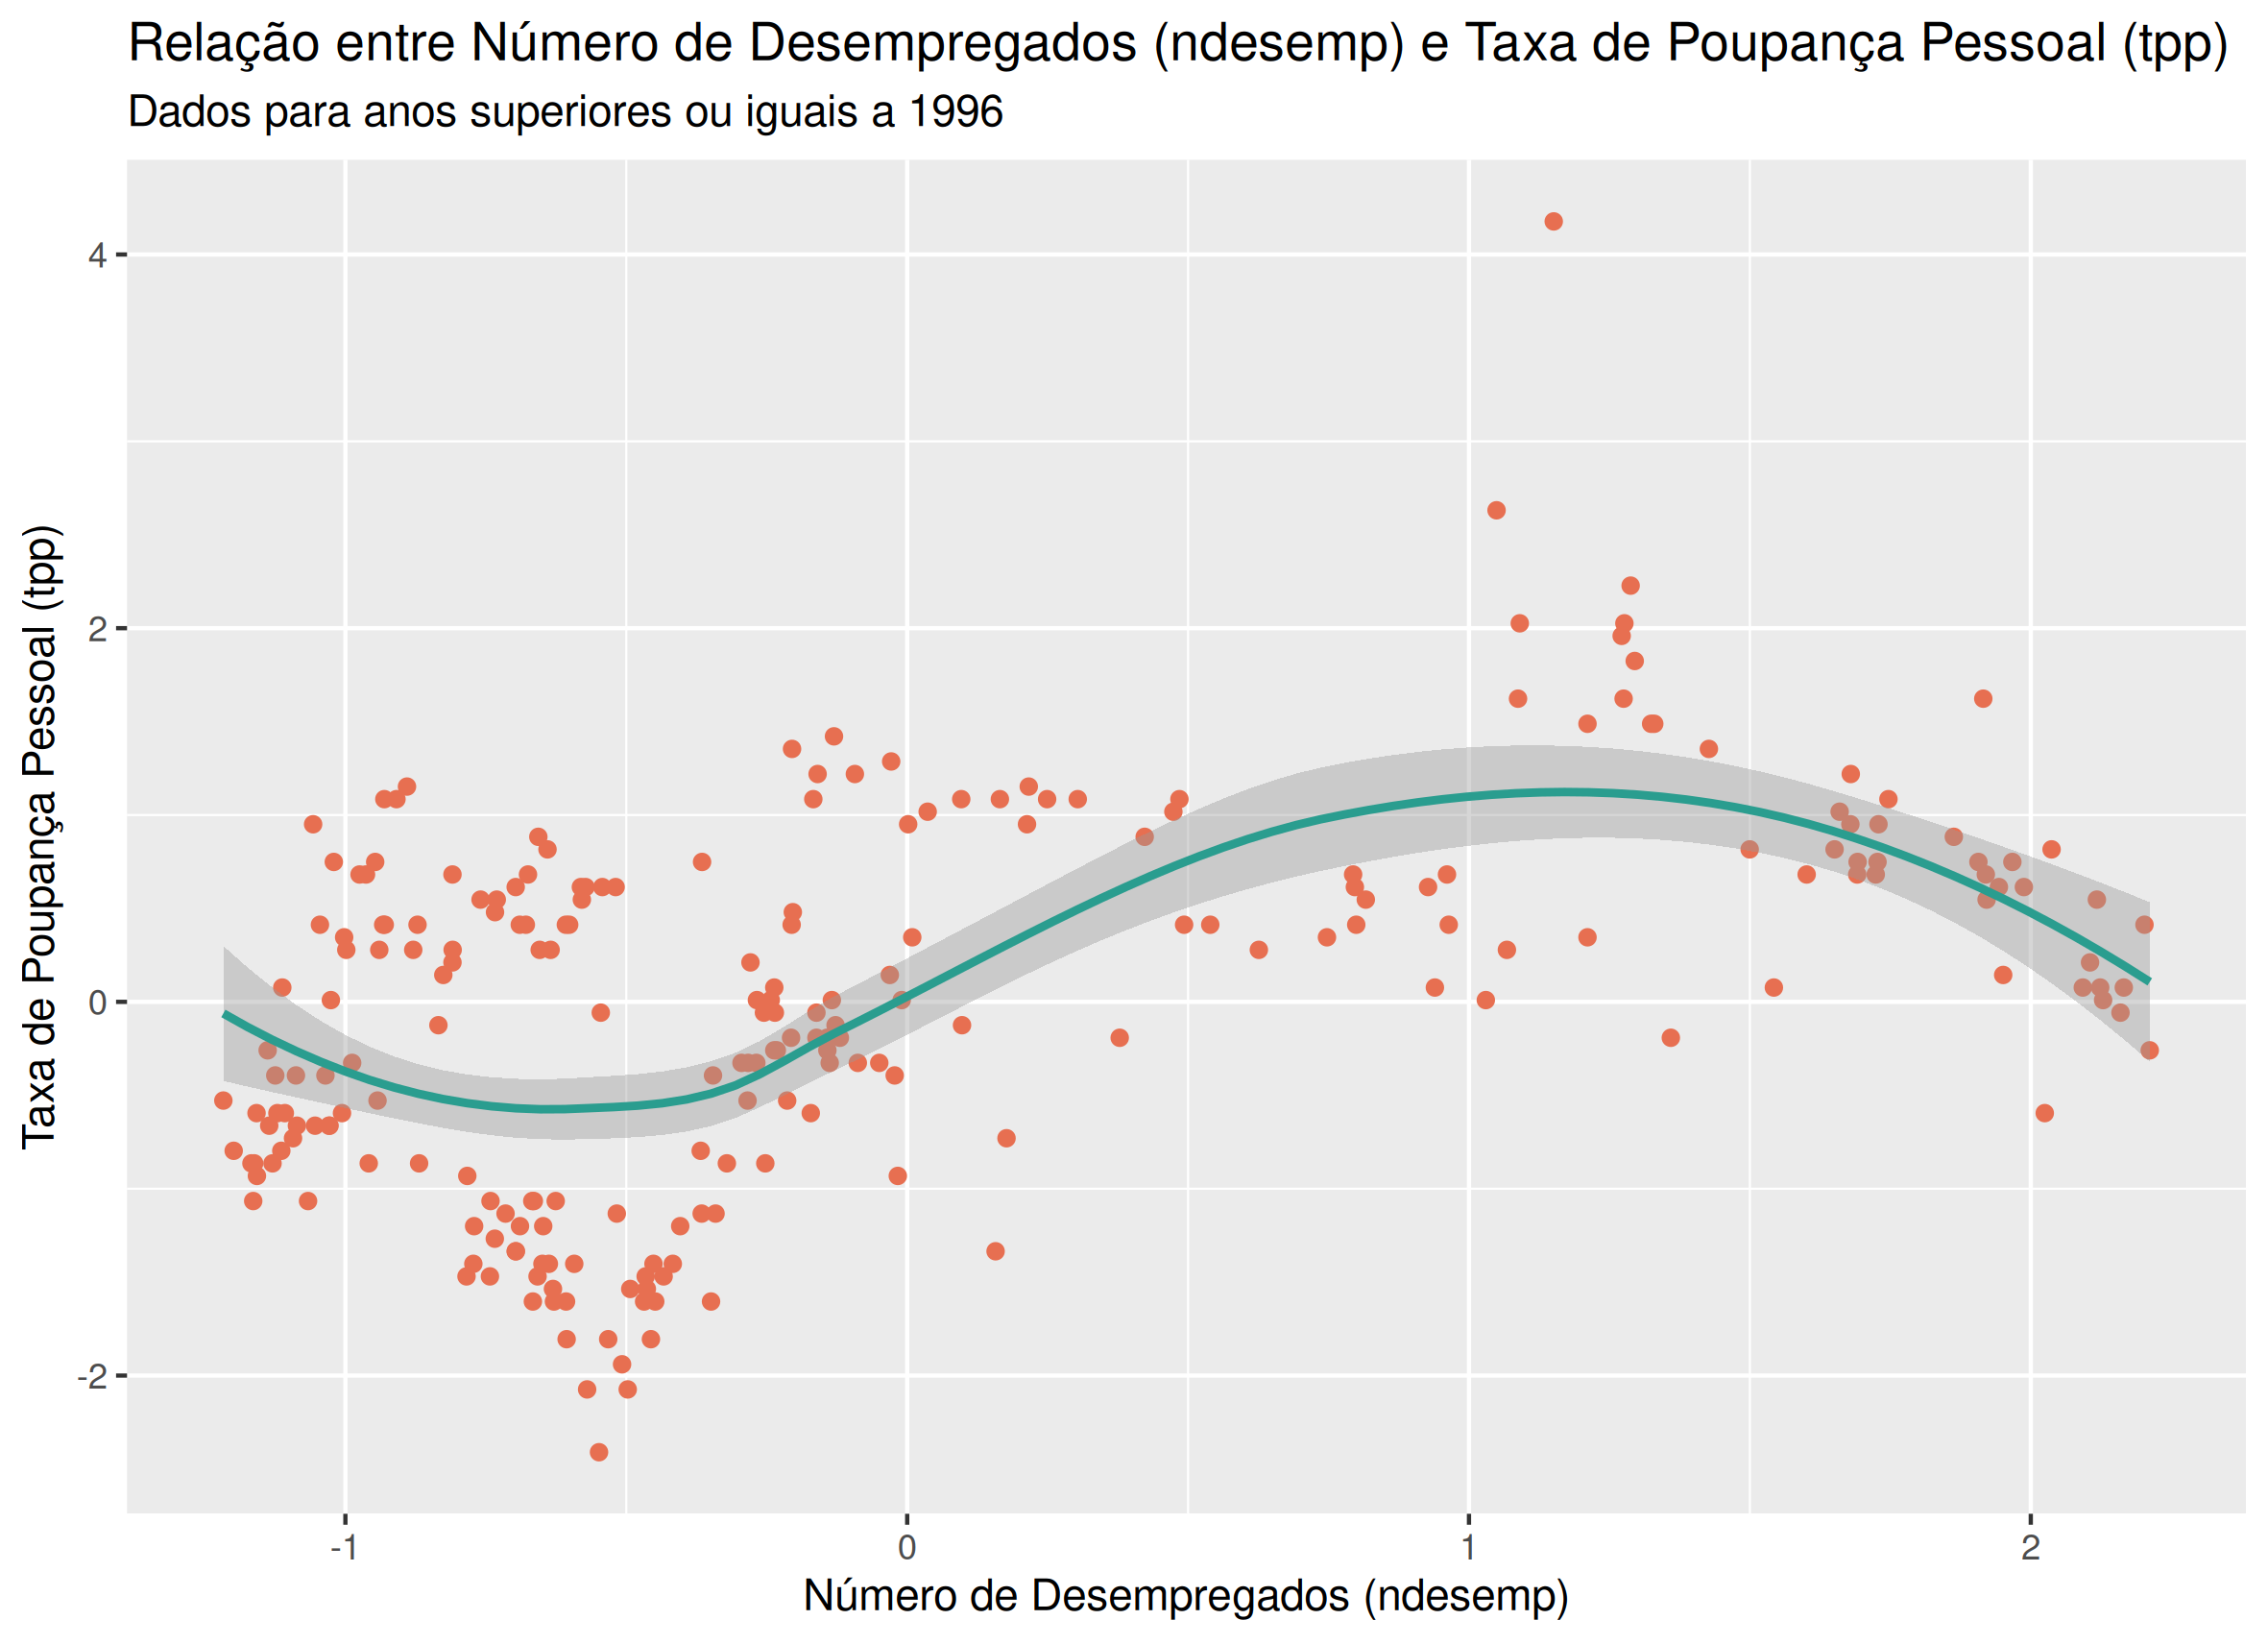
\includegraphics[scale = 0.8]{./ex01.png}
\end{figure}

\end{document}
